\documentclass[11pt]{report}

% !TeX document-id = {2870843d-1baa-4f6a-bd0a-a5c796104a32}
% !BIB TS-program = biber
% !TeX encoding = UTF-8
% TU Delft beamer template

\documentclass[aspectratio=43]{beamer}
\usepackage[english]{babel}
\usepackage{csquotes}
\usepackage{calc}
\usepackage[absolute,overlay]{textpos}
\usepackage{graphicx}
\usepackage{subfig}
\usepackage{mathtools}
\usepackage{amsfonts}
\usepackage{amsthm}
\usepackage{comment}
\usepackage{siunitx}
\usepackage{MnSymbol,wasysym}
\usepackage{array}
\usepackage{qrcode}

\setbeamertemplate{navigation symbols}{} % remove navigation symbols
\mode<presentation>{\usetheme[verticalbar=false]{tud}}

% BIB SETTINGS
\usepackage[
    backend=biber,
    giveninits=true,
    maxnames=30,
    maxcitenames=20,
    uniquename=init,
    url=false,
    style=authoryear,
]{biblatex}
\addbibresource{bibfile.bib}
\setlength\bibitemsep{0.3cm} % space between entries in the reference list
\renewcommand{\bibfont}{\normalfont\scriptsize}
\setbeamerfont{footnote}{size=\tiny}
\renewcommand{\cite}[1]{\footnote<.->[frame]{\fullcite{#1}}}
\setlength{\TPHorizModule}{\paperwidth}
\setlength{\TPVertModule}{\paperheight}

\newcommand{\absimage}[4][0.5,0.5]{%w
	\begin{textblock}{#3}%width
		[#1]% alignment anchor within image (centered by default)
		(#2)% position on the page (origin is top left)
		\includegraphics[width=#3\paperwidth]{#4}%
\end{textblock}}

\newcommand{\mininomen}[2][1]{{\let\thefootnote\relax%
	\footnotetext{\begin{tabular}{*{#1}{@{\!}>{\centering\arraybackslash}p{1em}@{\;}p{\textwidth/#1-2em}}}%
	#2\end{tabular}}}}

\title{%
    A report \\
    \large WI4204 - Advanced Modelling
}
\author{Philip Soliman (4945255), Auke Schaap (4457919)}
\date{April 2023}

\begin{document}
\maketitle

\begin{abstract}
    This is the abstract.

    \todo{Philip: Citations in Introduction}
    \todo{Philip: final check}
    \todo{Philip: Rewriteshite}

    Due to the wide adoption of solar panels, electic vehicles, and other technologies, the energy supply and consumption in Netherlands has changed drastically. This has led to a change in the load profile of the distribution transformers, which are used to step down the voltage from the medium voltage grid to the low voltage grid. 
    Currently, models do not accurately reflect the behaviour of the transformers under these new conditions. 
    This paper presents a model that can accurately model the magnetic field without assuming a sinusoidal source current. The model can be used to model any frequency, as well as multiple frequencies. The model also correctly captures the behaviour of the core at loads close to the saturation point, by including the non-linear permeability of the core material.
    These are both improvements over the current linear models, which are not able to capture these behaviours.

\end{abstract}
\chapter{Introduction}

Over the last few years, the energy supply and consumption in the Netherlands has changed drastically. For example, there has been an increase in energy generated by solar panels, as well as an increase in the number electric vehicles on roads \cite{vanDijk2022}. 
Both the solar panels on people's roofs as well the charging docks for their electric vehicles introduce higher harmonics into the electricity grid \cite{energietransitie}, \cite{energieVerbenCons}.
These higher harmonics increase the load on distribution transformers, which causes overheating, degraded performance and decreased lifetime \cite{vanDijk2022}

Distribution transformers are used to transform the high voltage electricity from the transmission grid to a lower voltage for the end-user.
In this process, some of the electrical potential energy is dissipated as heat. 

In modelling these losses, we can assume the magnetic field in the core to have the same temporal behavior as the the load on the transformer; sinusoidal with the same frequency. 
This works for load profiles with multiple frequencies, as long as the magnetic permeability of the core is assumed constant.

However, the magnetic permeability $\mu$ of the core is only constant by approximation. In reality $\mu$ depends on the magnetic field strength, which introduces non-linearities in the governing equations.
For low harmonics, i.e. $50$ Hz, these non-linearities are negligible.
For higher harmonics, the skin-effect causes the magnetic flux to be concentrated near the edges of the transformer. 
The flux in these edge regions is then high enough that $\mu$ can no longer be assumed to be constant. 
This results in a model error for higher harmonics.

Additionally, the superposition of the magnetic field resulting from several load frequencies is no longer valid for non-linear systems.
This is because each of the frequencies are now coupled to each other, through $\mu$'s dependence on the magnetic field strength.

This paper aims to model the magnetic field in a distribution transformer, taking into account the non-linearities introduced by higher frequencies and loads.
The proposed model makes no assumptions on the frequency of the magnetic field resulting from a load profile containing (multiple) higher harmonics.

\Cref{sec:background} explains relevant background information. 
In \cref{sec:model}, the model is derived. 
Then, \cref{sec:results} presents the results of the model. 
Lastly, \cref{sec:discussion} discusses the results and the model.


\chapter{Background} \label{sec:background}

This chapter provides some background theory on the problem. It describes the electrical grid, the function of a transformer, 
the effect of modern appliances on the transformer and modelling of this effect. It draws heavily from the work of \cite{vanDijk2022}.

\section{Electrical grid}
\label{sec:grid}
Power generated at dams, nuclear power- and coal plants is transmitted to the consumer through the electrical grid. The grid is a network of power lines, transformers and other equipment. 
The grid is divided into three parts: generation, transmission and distribution. All these components are displayed in
figure \ref{fig:grid}.
\begin{figure}[H]
    \centering
    
\includegraphics[width=0.5\textwidth]{img/distribution grid.png}
    \caption{Electricity grid \cite{mBizon2010}.}
    \label{fig:grid}
\end{figure} 
In the Netherlands specifically, the grid is divided into three voltage levels: extra high voltage, high voltage and low voltage.
The transmission grid ensures this high voltage ends up at factories, large power transformers and additional power is extracted from industrial and medium sized power plants.
Moreover, it is managed by a Transmission System Operator (TSO). 

Similarly, the distribution grid connects the transmission grid, cities, the rural network, solar-, wind farms to each other. It, in turn is managed by a Distribution System Operator (DSO)
In this paper the focus is on the transformers in the distribution grid. Figure \ref{fig:transformer} shows an example of such an transformer. This is because the distribution grid is the last part of the grid before the consumer. 
Consequently, the effects of modern appliances are most prominent in these types of transformers.
\begin{figure}[H]
    \centering
    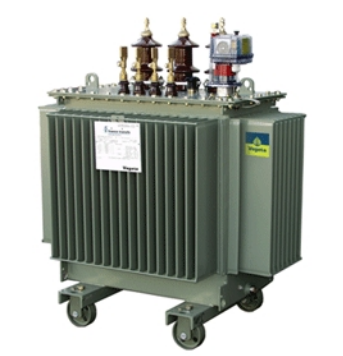
\includegraphics[width=0.5\textwidth]{img/transformer.png}
    \caption{Transformer \cite{dGebouwd2021}}
    \label{fig:transformer}
\end{figure}
The main goal of any transformer is to allow for the transmission of electrical energy over long distances. 
It achieves this by either increasing or decreasing voltage. In the former case, it is called a step-up transformer, in the latter case a step-down transformer.
A step-up tranformer allows for long distance transmission of electrical energy because the power loss is proportional to the current squared, which is decreased for increased voltage.
On the other hand, a step-down transformer is used to decrease the voltage to a level that is safe for the end-consumer.

\section{Workings of transformer}
A transformer is a device that transfers electrical energy from one circuit to another through inductively coupled conductors. 
It has three main components: a primary coil, a secondary coil and a core (see Figure \ref{fig:transformercore}). 
The primary coil is connected to the source of the electrical energy, the secondary coil is connected to a load and the core is made from a ferromagnetic material.
In the case of a distribution transformer, the primary coil is connected to the transmission grid and the secondary coil is connected to the distribution grid.
\begin{figure}[H]
    \centering
    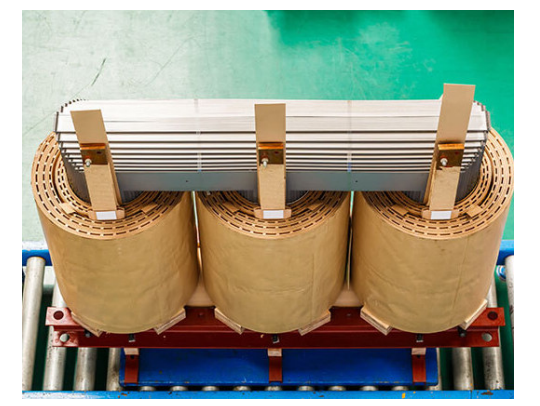
\includegraphics[width=0.5\textwidth]{img/transformercore.png}
    \caption{Main components of a transformer: primary (outer) coil, secondary (inner) coil and core. The coils are wound around the core
    and are wrapped in insulation themselves (\cite{sSatsangi}).}
    \label{fig:transformercore}
\end{figure}

The insulation around the coils is necessary to prevent short-circuiting. Hence the lifetime of a transformer is limited by the lifetime of the insulation.
The latter in turn is determined by the amount of heat generated in the transformer. This heat is dissiapted through the core and the coils, where the core is the main contributor.
Therefore, this paper focusses on modelling the magnetic field generated in the core. 
The core losses and subsequent temperature profile may then be calculated from this magnetic field using the Steinmetz equation (\cite{steinmetzEq,vanDijk2022}).

\section{Higher Harmonics}
As stated in Section \ref{sec:grid}, the effect of modern appliances like computers, LEDs, solar panels and electric cars is most prominent in the distribution grid.
LEDs, for instance, are non-linear loads, which means they draw a current that is composed of a fundamental frequency and higher harmonics.
These higher harmonics are multiples of the fundamental frequency. The effect of these higher harmonics is that the current is no longer sinusoidal, but has a distorted shape.
This distortion is shown in Figure \ref{fig:higherharmonics}.
\begin{figure}[H]
    \centering
    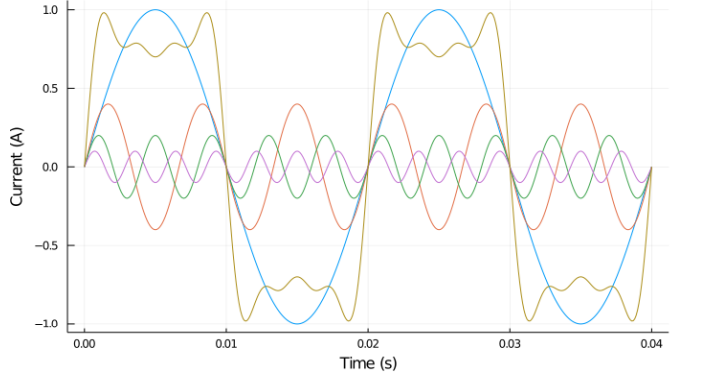
\includegraphics[width=0.5\textwidth]{img/higher_harmonics.png}
    \caption{Distorted current waveform (\cite{vanDijk2022}).}
    \label{fig:higherharmonics}
\end{figure}
The magnetic field in the core depends on the frequency. A concrete example of this is the skin effect, which is the tendency of an alternating electric current to become distributed within a conductor such that the current density is largest near the surface of the conductor, and decreases with greater depths in the conductor. The depth at which the current density is 37\% of the current density at the surface is called the skin depth. It is given by (\cite{skinEffect})
\begin{equation}
    \delta = \sqrt{\frac{2 \rho}{\omega \mu}} = \sqrt{\frac{\rho}{\pi f \mu_0 \mu_r}},
\end{equation}
where:
\begin{itemize}
    \item $\rho$: The resistivity of the conductor. For an iron core, this is taken as $\rho = 9.71 \cdot 10^{-8}$ $\Omega \! \cdot \! \text{m}$ (\cite{restitivity}).
    \item $\mu$: The permeability of the conductor, given by $\mu_r \mu_0$.
    \item $\mu_r$: The relative magnetic permeability of the conductor. For an iron core, this is somewhere around $10^3$. Therefore, this is chosen as $\mu_r = 1000$.
    \item $\mu_0$: The permeability of free space. This is generally taken as $\mu_0 = 4 \pi \cdot 10^{-7}$ $\text{H/m}$.
    \item $\omega$: The angular frequency of current, given by $2 \pi f$, where $f$ is the frequency. This is variable in our case.
\end{itemize}
This becomes smaller for higher frequencies, and is hence more prominent for higher harmonics. Therefore, higher harmonics lead to an increased core loss. A numerical result is given in \cref{tab:skin_effect}.

\begin{table}
    \centering
    \begin{tabular}{l|l}
        Frequency & $\delta$ (mm) \\
        \hline
        50 Hz   & 0.701 mm \\
        100 Hz  & 0.496 mm \\
        150 Hz  & 0.351 mm \\
        500 Hz  & 0.222 mm \\
        1000 Hz & 0.157 mm \\
    \end{tabular}
    \caption{Numerical values for the skin effect at different frequencies, with parameters as described below.}
    \label{tab:skin_effect}
\end{table}


\section{Permeability of the core}
Another complication in modelling the magnetic field in the core is that the permeability of the core is not constant for sufficiently large magnetic fields.
This is called the saturation of the core. The permeability of the core is given by
\begin{equation}
    \mu = \mu_0 \mu_r,
\end{equation}
where $\mu_0$ is the permeability of free space and $\mu_r$ is the relative permeability of the core. The permeability is a function of the magnetic field strength $H$.
The magnetic field strength is given by
\begin{equation}
    H = \frac{B}{\mu},
\end{equation}
where $B$ is the magnetic flux density. 

From this it follows that we can derive $\mu$ given we know the relation between $B$ and $H$. 
This relation is called the B-H curve, an example of which is visible in Figure \ref{fig:bhcurve}.
\begin{figure}[H]
    \centering
    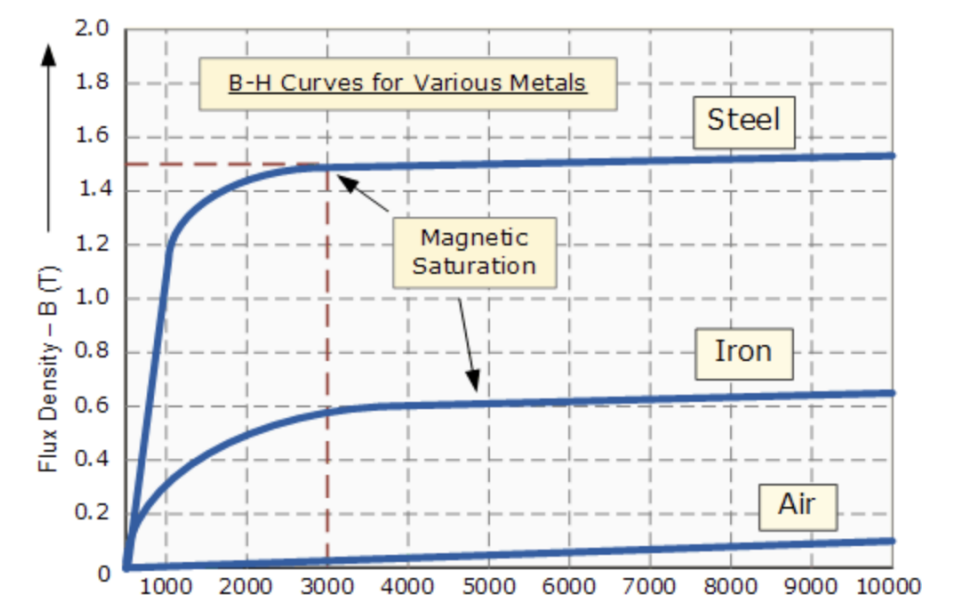
\includegraphics[width=0.5\textwidth]{img/BH_curve.png}
    \caption{B-H curve for various metals. $\mu$ is the slope of this curve. Once $\mu$ becomes nearly zero, the material is said 
    to be the saturated \cite{bhcurve}.}
    \label{fig:bhcurve}
\end{figure}


\chapter{Model} \label{sec:model}
This chapter describes the model used to simulate the magnetic field in the transformer core. The implementation is available at \url{https://github.com/aukeschaap/am-transformers}.

\section{Problem derivation}

To define the problem, we start with the Maxwell equations and corresponding constitutive relations. The Maxwell equations are given by
\begin{align*}
    \nabla \times \mathbf{E} &= -\frac{\partial \mathbf{B}}{\partial t}, \\
    \nabla \times \mathbf{H} &=  \mathbf{J} + \frac{\partial \mathbf{D}}{\partial t}, \\
    \nabla \cdot \mathbf{B} &= 0, \\
    \nabla \cdot \mathbf{D} &= \rho,
\end{align*}
where
\begin{itemize}
    \item $\mathbf{E}, [V/m]$ is the electric field intensity,
    \item $\mathbf{H}, [A/m]$ is the magnetic field intensity,
    \item $\mathbf{J}, [A/m^2]$ is the current density,
    \item $\mathbf{B}, [T]$ is the magnetic flux density,
    \item $\mathbf{D}, [C/m^2]$ is the electric flux density,
    \item $\rho, [C/m^3]$ is the free charge density.
\end{itemize}

\noindent These have the following constitutive relations:
\begin{align*}
    \mathbf{J} &= \mathbf{J_e} + \mathbf{J_c} \\
    \mathbf{B} &= \mu\mathbf{H} \\
    \mathbf{J}_c &= \sigma\mathbf E \\
    \mathbf{D} &= \epsilon \mathbf E
\end{align*}
where
\begin{itemize}
    \item $\mathbf{J_e}$ is the external current density,
    \item $\mathbf{J_c}$ is the conduction current density,
    \item $\sigma$ is the conductivity of the material,
    \item $\mu = \mu_0\mu_r$ is the permeability of the core,
    \item $\epsilon = \epsilon_0\epsilon_r$ is the permittivity of the material.
\end{itemize}

\begin{assumption}
    The permittivity of vacuum $\epsilon_0$ is very small, $(\mathcal{O}(10^{-12}))$, and for all materials in this research $\epsilon_r < 10$, so $\epsilon$ can be neclegted. Therefore, $\mathbf{D} \approx 0$ and can be neglected.
\end{assumption}

\noindent Substituting this in the Maxwell equations yields three equations,
\begin{align*}
    \nabla \times \mathbf{E} &= -\frac{\partial \mathbf{B}}{\partial t}, \\
    \nabla \times \left[\mu^{-1}\mathbf{B}\right] &=  \mathbf{J_e} + \sigma \mathbf{E}, \\
    \nabla \cdot \mathbf{B} &= 0.
\end{align*}

\noindent Using the potential formulation,
\begin{align*}
    \mathbf{E} &= -\nabla \varphi -\frac{\partial \mathbf{A}}{\partial t}, \\
    \mathbf{B} &= \nabla \times \mathbf A,
\end{align*}
we can formulate a system that we can solve.

\begin{assumption}
    We assume that the contribution of the electrostatic field $\varphi$ is negligble compared to the contribution of the potential field $\mathbf A$. That is, $\nabla \varphi = 0$, which implies that $\mathbf{E} = -\frac{\partial \mathbf{A}}{\partial t}$.
\end{assumption}

\begin{assumption}
    The flow of current is oriented along the $z$ axis, and the geometry is in the $xy$ plane. That is, $\mathbf{A} = (0, 0, A_z)$ and $\mathbf{J_e} = (0, 0, J_z)$. This implies $\nabla \times \mathbf A = (\partial_y A_z, -\partial_x A_z,0)$.
\end{assumption}

\noindent Substituting these assumptions into the Maxwell equations and rearranging, we obtain our problem definition.
\begin{equation*}
    \sigma\frac{\partial A_z}{\partial t} = - \left(\frac{\partial}{\partial x}\left[\frac{1}{\mu} \frac{\partial A_z}{\partial x}\right] + \frac{\partial}{\partial y}\left[\frac{1}{\mu} \frac{\partial A_z}{\partial y}\right]\right) + J_z,
\end{equation*}

\begin{problem}
    Find $A_z$ in the system
    \begin{equation}
        \sigma\frac{\partial A_z}{\partial t} = - \nabla \cdot \left(\frac{1}{\mu} \nabla A_z \right) + J_z,
    \end{equation}
    where
    \begin{itemize}
        \item $A_z$ is the magnetic vector potential in the $z$ direction,
        \item $\mu$ is the permeability of the core,
        \item $J_z$ is the imposed source current density,
        \item $\sigma$ is the conductivity of the core.
    \end{itemize}
    From this point onwards, this will be formulated as
    \begin{equation}
        \sigma\dot u = \nabla \cdot \left[\frac{1}{\mu}\nabla u\right] + f.
    \end{equation}
\end{problem}

\newpage
\section{Spatial discretisation using finite element method}

\begin{figure}
    \centering
    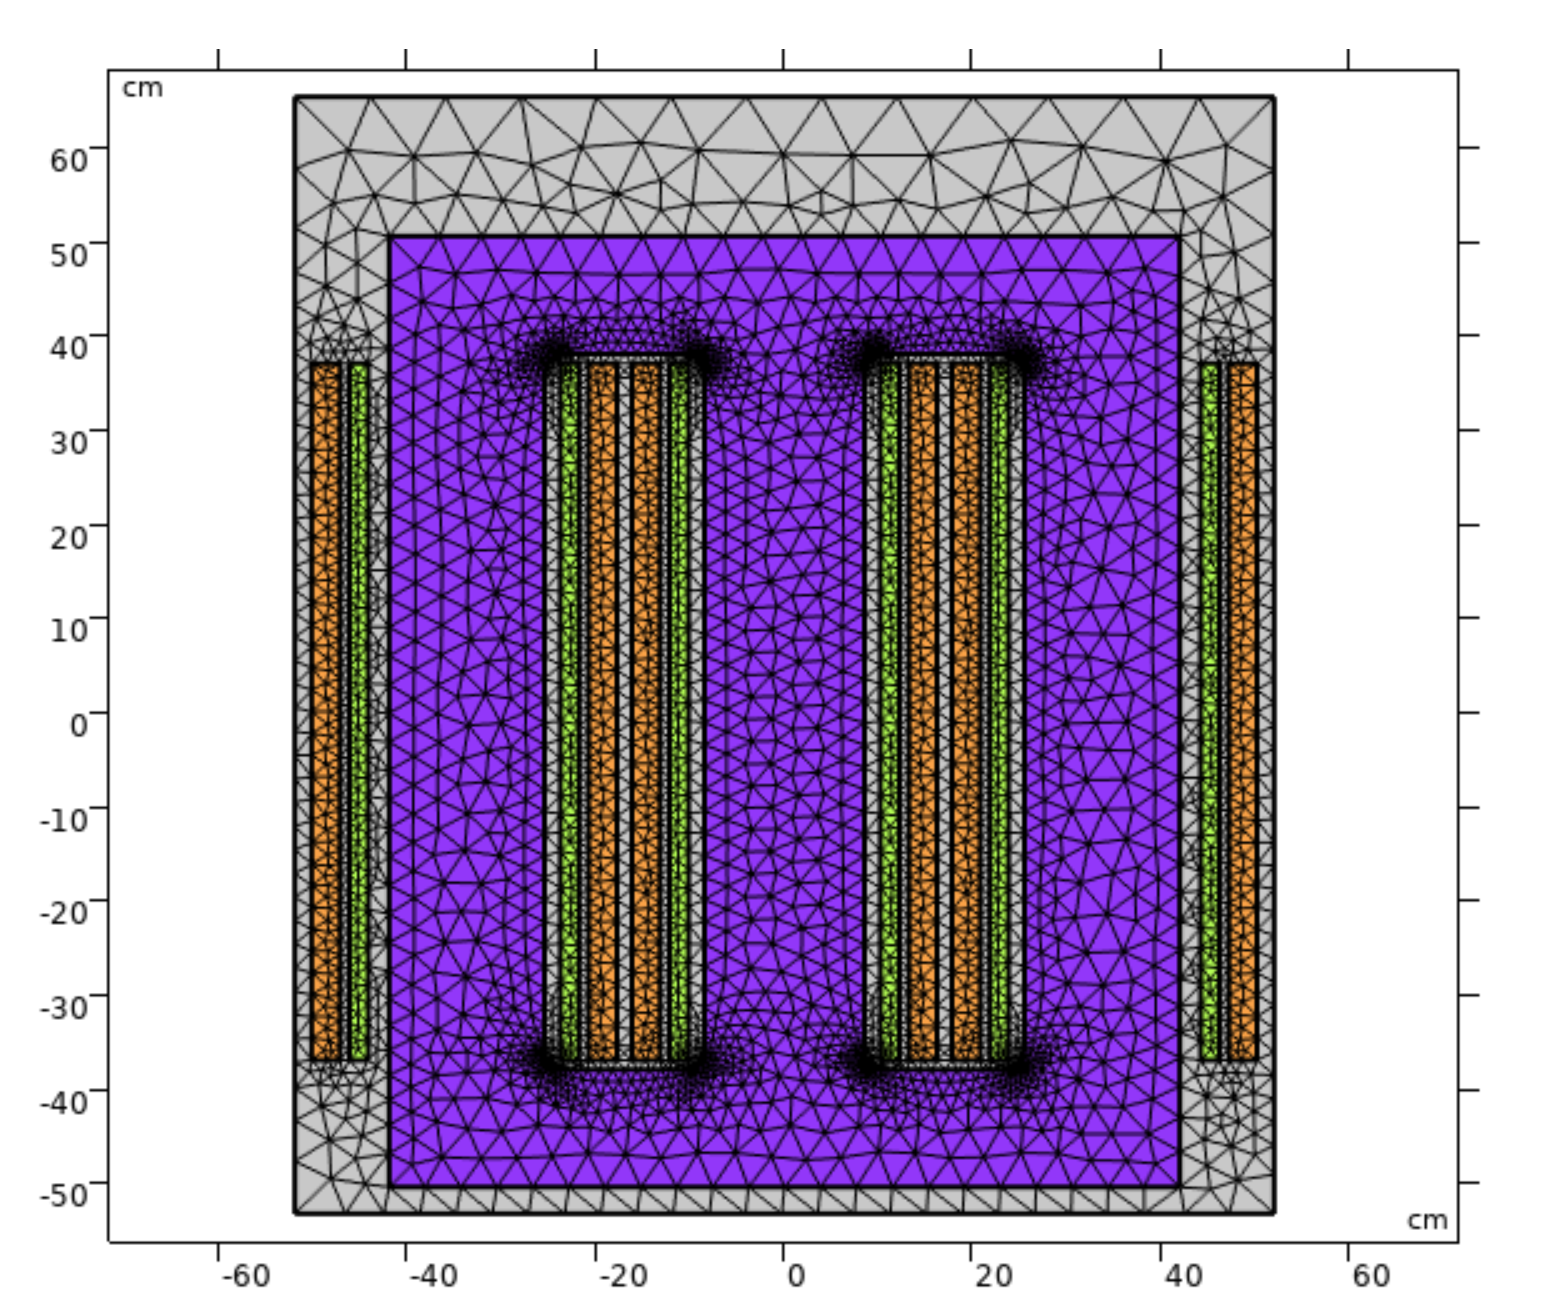
\includegraphics[width=0.5\textwidth]{img/regular_mesh.png}
    \caption{The mesh used to discretize the domain (\cite{vanDijk2022}).}
    \label{fig:regular_mesh}
\end{figure}

To solve this system, the finite element method can be used. Choosing a first order basis function 
\[
    \phi_i = a_i + b_i x + c_i y,
\]
for each node $i$, the solution $u$ can be approximated as
\[
    u = \sum_{i=1}^N u_i \phi_i.
\]
This results in the following weak form.
\begin{weakform}
    \begin{equation}
        \sigma M \dot u = K(\mu(u)) u + f,
        \label{eqn:weakform}
    \end{equation}
    where
    \begin{itemize}
        \item $u$ is $A_z$, the solution.
        \item $M$ is the mass matrix,
        \item $K$ is the stiffness matrix,
        \item $f$ is the source term, given by $J_z$,
    \end{itemize}
\end{weakform}

\noindent The mass matrix on element $e_k$,  $M_{e_k}$ is given by
\begin{align*}
    M_{e_k} = \left[\int_{\Omega_{e_k}}\phi_i\phi_j d\Omega \right]_{1 \leq i, j \leq 3}
\end{align*}

\noindent Similarly, the local stiffness matrix $K_{e_k}$ is given by
\begin{align*}
    K_{e_k}(\mu(u)) &= \left[\int_{\Omega_{e_k}} \phi_i \nabla \cdot \left(\frac{1}{\mu} \nabla \cdot \phi_j \right) d \Omega \right]_{1 \leq i, j \leq 3} \\
    &= -\int_{\Omega_{e_k}} \frac{1}{\mu} \nabla \phi_i \nabla \phi_j d \Omega
\end{align*}

\noindent Similarly the local source term $f_{e_k}$ is given by
\begin{align*}
    f_{e_k}(t) = \left[\int_{\Omega_e} f(x,y,t) \phi_i d \Omega\right]_{1 \leq i \leq 3}\\
\end{align*}

\noindent We can exactly calculate the integrals using the following quadrature rule for first order polynomials.
\begin{align*}
    \int_{\Omega_e}g(x,y)dxdy = A_{e_k}\bar{g}_{e_k}, \\
\end{align*}
where $A_{e_k}$ is the area of element $e_k$ and $\bar{g}_{e_k}$ is the average of function $g$ over element $e_k$.

\subsection{Time dependence}
If $\mu$ is constant we may write $K(\mu(u)) = K(\mu) = \frac{1}{\mu}K$. In this case the use of separation of variables is valid. 
If $\mu$ is dependent on $u$, separation of variables is not valid due to the non-linear nature of the problem. 
In this case a time stepping method is necessary. This section outlines both approaches and their implementation.
Ultimately, the time stepping method is used, because the permeability this paper is concerned with the non-linear case.

\subsection{Separation of variables}
Applying separation of variables
\begin{align*}
    u(x,y,t) = \hat u(x,y) \cdot e^{j\omega t}.
\end{align*}
to the weak form \eqref{eqn:weakform} yields
\begin{equation*}
    \left[\sigma \omega j M + \frac{1}{\mathbf \mu}A\right]\hat u = \hat f.
\end{equation*}
This is a linear system of equations, which can be solved using a linear solver. 
Additionally it may be solved for multiple frequencies $\omega_1, \omega_2, \dots$ by writing
\begin{equation}
    u(x,y,t) = \hat u_1(x,y) e^{j\omega_1 t} + \hat u_2(x,y) e^{j\omega_2 t} + \dots,
\end{equation}
solving the above system for each frequency, and summing the solutions. However it must be noted that the influence of the frequencies on each other is not taken into account in this approach.
This is why the time stepping method is used in this paper.

\subsection{Time stepping}
The time derivative in equation \ref{eqn:weakform} can be approximated using a backward Euler method, 
\begin{equation*}
    \sigma M\frac{u^{k} - u^{k-1}}{\Delta t} = K(u^{k}) u^{k} + f^{k},
\end{equation*}
where $u^k$ is the solution at time $t^k$ and $u^{k+1}$ is the solution at time $t^{k+1} = t^k + \Delta t$.
This leads to the following implicit time stepping scheme.
\begin{equation*}
    \left[\sigma M - \Delta t K(u^{k-1})\right]u^{k} = \sigma M u^{k-1} + \Delta t f^{k}.
\end{equation*}
During each time step, this non-linear system of equations must be solved. This is done using an iterative scheme with dampening factor $\alpha$. This means that instead of $u^k_i$, there is $\tilde{u}^k_i$, defined by
\begin{equation*}
    \tilde{u}^k_{i} = \alpha \tilde{u}^k_{i-1} + (1-\alpha)u^k_{i-1},
\end{equation*}
where the superscript $k$ denotes time, and subscript $i$ denotes the iteration number. This is then used for solving the system of equations for $u^k_i$:
\begin{equation}
    \left[\sigma M - \Delta t K(\tilde{u}^k_{i})\right] u^k_{i} = \left[\sigma M \tilde{u}_{i}^{k} + \Delta t f^{k}\right].
\end{equation}

\noindent This is repeated until the residual is sufficiently small. That is
\begin{equation*}
    ||u^k_{i-1} - u^{k}_i||_2 \leq \epsilon,
\end{equation*}
where $\epsilon$ is a small number. In this paper $\epsilon = 10^{-3}$ is used. The full algorithm is given in Algorithm \ref{alg:time_stepping}.


\begin{algorithm}
    \caption{\label{alg:time_stepping} Time-stepping algorithm using Backward Euler}
    \begin{algorithmic}[1]
    \Function{nonlinear-solve}{}
    \State $u^0 \leftarrow \textbf{0}$
    \For{$k \in [0, N_t]$}{}
        \State $i \leftarrow 0$
        \State $u^k_0 \leftarrow u^{k-1}$
        \State $\tilde{u}^k_0 \leftarrow u^{k-1}$
        \While{$\Delta u \leq \epsilon$}{}
            \State $i \leftarrow i + 1$
            \State $\tilde{u}^k_{i} \leftarrow \alpha \tilde{u}^k_{i-1} + (1-\alpha)u^k_{i-1}$
            \State $u^k_{i} \leftarrow \left[\sigma M - \Delta t K(\tilde{u}^k_{i})\right]^{-1}\left[\sigma M \tilde{u}_{i}^{k} + \Delta t f^{k}\right]$
            \State $\Delta u \leftarrow ||u^k_{i-1} - u^{k}_i||_2$
        \EndWhile
        \State $u^{k+1} \leftarrow u^k_i$
    \EndFor
    \EndFunction
    \end{algorithmic}
\end{algorithm}
\chapter{Results} \label{sec:results}

Some results here.

\begin{figure}[t]
    \centering
    \includegraphics[width=0.8\textwidth]{phaseplot_of_B.eps}
    \caption{Phase plot of $B$}
    \label{fig:phaseplot_of_B}
\end{figure}
\chapter{Discussion} \label{sec:discussion}


\section{Conclusion}
From the results presented in \autoref{sec:results}, we can conclude the following.

Firstly, the method is able to model the transformer core in a way that is consistent with the physical properties of the core material. This is shown by the fact that the magnetic flux density in the core is inversely proportional to the permeability of the core material. Consequently, the model correctly captures the behaviour of the core at loads close to the saturation point, as seen by the fact that the magnetic flux density in the core is constant across the cross section of the core. This directly shows that the linear model is not able to capture the behaviour of the core at loads close to the saturation point.

Furthermore, this model does not make any assumptions on the underlying frequency of the source current. As a result, the model can also be used to model higher frequencies, as well as multiple frequencies, correctly. As the non-linearities disallow separation of variables in the frequency domain, this is an improvement over the previous work. \todo{Rewrite}

\section{Future work}
The model presented in this paper is a first step towards a more accurate model of the magnetic field in a distribution transformer. However, there are still some improvements that can be made.
\vspace{5pt}

% Frequencies
\noindent This paper only presents results for a single frequency. In theory, the model is also valid for higher, as well as multiple frequencies. However, the model is not yet validated for these cases. Therefore, more research is needed to determine the validity of the model for these cases.

% Optimization
\vspace{5pt}
\noindent At this moment, the model is not fully optimized. As a result, the execution time is quite long. If this is to be used to model a longer time horizon, the execution time needs to be reduced. Some steps in this direction have already been taken:
\begin{itemize}
    \item Matrices have been implemented in a sparse format, which reduces the memory usage and the number of operations needed to perform the matrix-vector multiplications.
    \item A data structure \verb|FastSparse| has been implemented, that efficiently allocates memory for initializing the (sparse) matrices $M$ and $K$.
    \item The assembly of the matrices $M$ and $K$ has been optimized to use to least amount of memory allocations possible.
\end{itemize}
However, there are still some steps that can be taken to further reduce the execution time:
\begin{itemize}
    \item Efficient linear system solver: the current linear system solver is not very efficient. This could be an iterative method, or a Krylov subspace method.
    \item Backward Euler is used to time-step. This could be done more accurately by using a higher order method, such as the Runge-Kutta method, further improving execution time.
\end{itemize}


% Parameter analysis
\vspace{5pt}
\noindent Furthermore, the parameters used in the model are not in agreement with reality. For instance, the core does not operate close to saturation in reality, but at much lower flux densities. Most parameters are estimated based on \cite{vanDijk2022}, and might therefore not be accurate. More research is needed to determine the correct parameters.

% Hybrid mesh
\vspace{5pt}
\noindent Finally, the mesh used in this paper can be improved. The mesh used in this paper is a triangular mesh, and lacks detail to correctly address the skin effect that arises at higher frequencies. \Cref{tab:skin_effect} shows the skin effect for different frequencies. As can be seen, the skin effect is not present at $50$ Hz, but its contribution increases with frequency. Therefore, a hybrid mesh can be used, where the mesh is refined near the edges of the transformer, where the skin effect is most prominent. This will increase the accuracy of the model at higher frequencies. This mesh is shown in \cref{fig:mesh_hybrid}.

\begin{figure}
    \centering
    \begin{multicols}{2}
        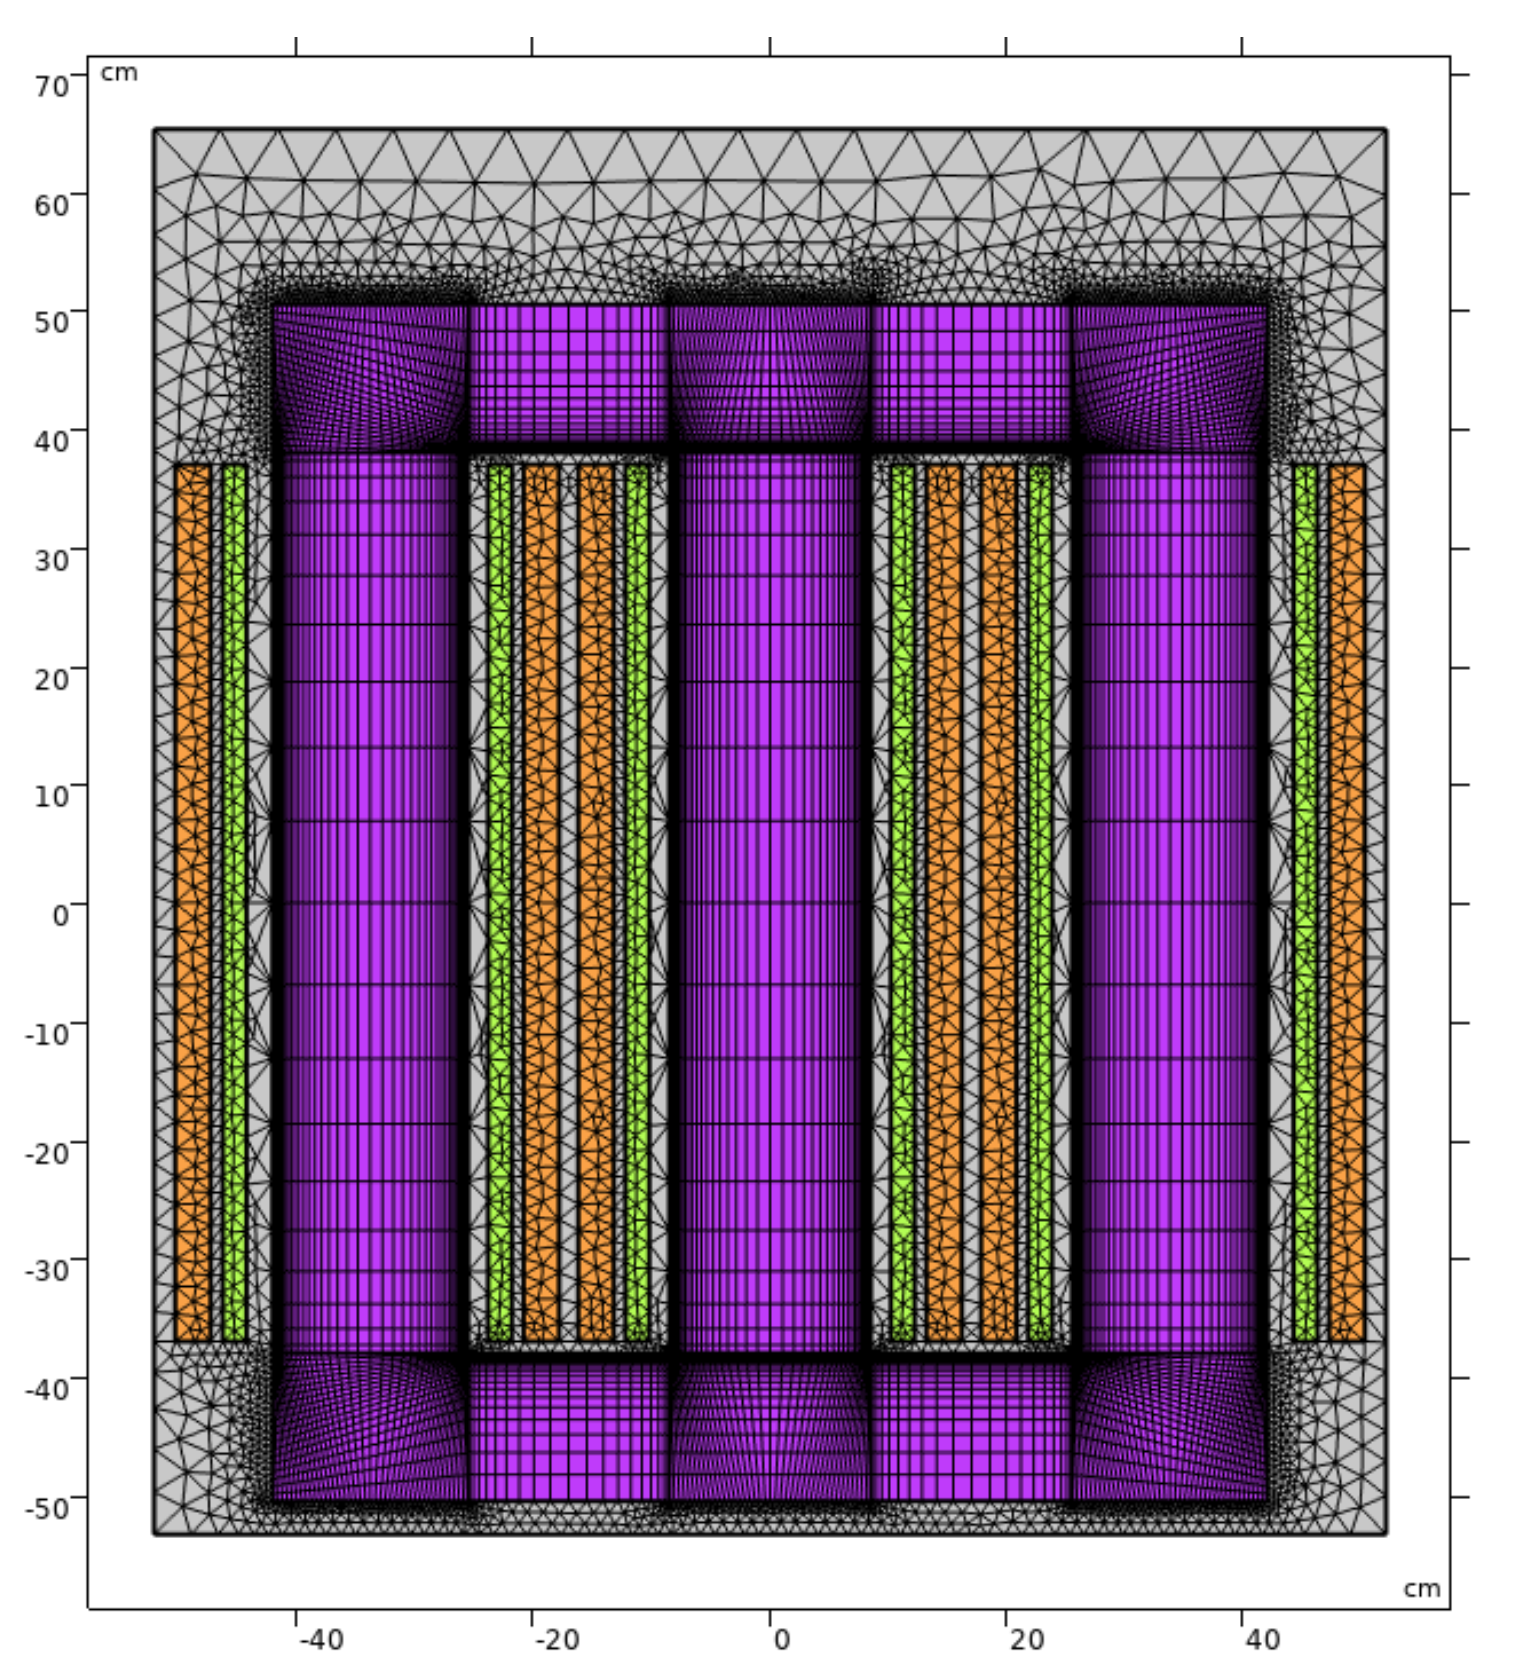
\includegraphics[width=0.45\textwidth]{img/hybrid_mesh_full.png}
        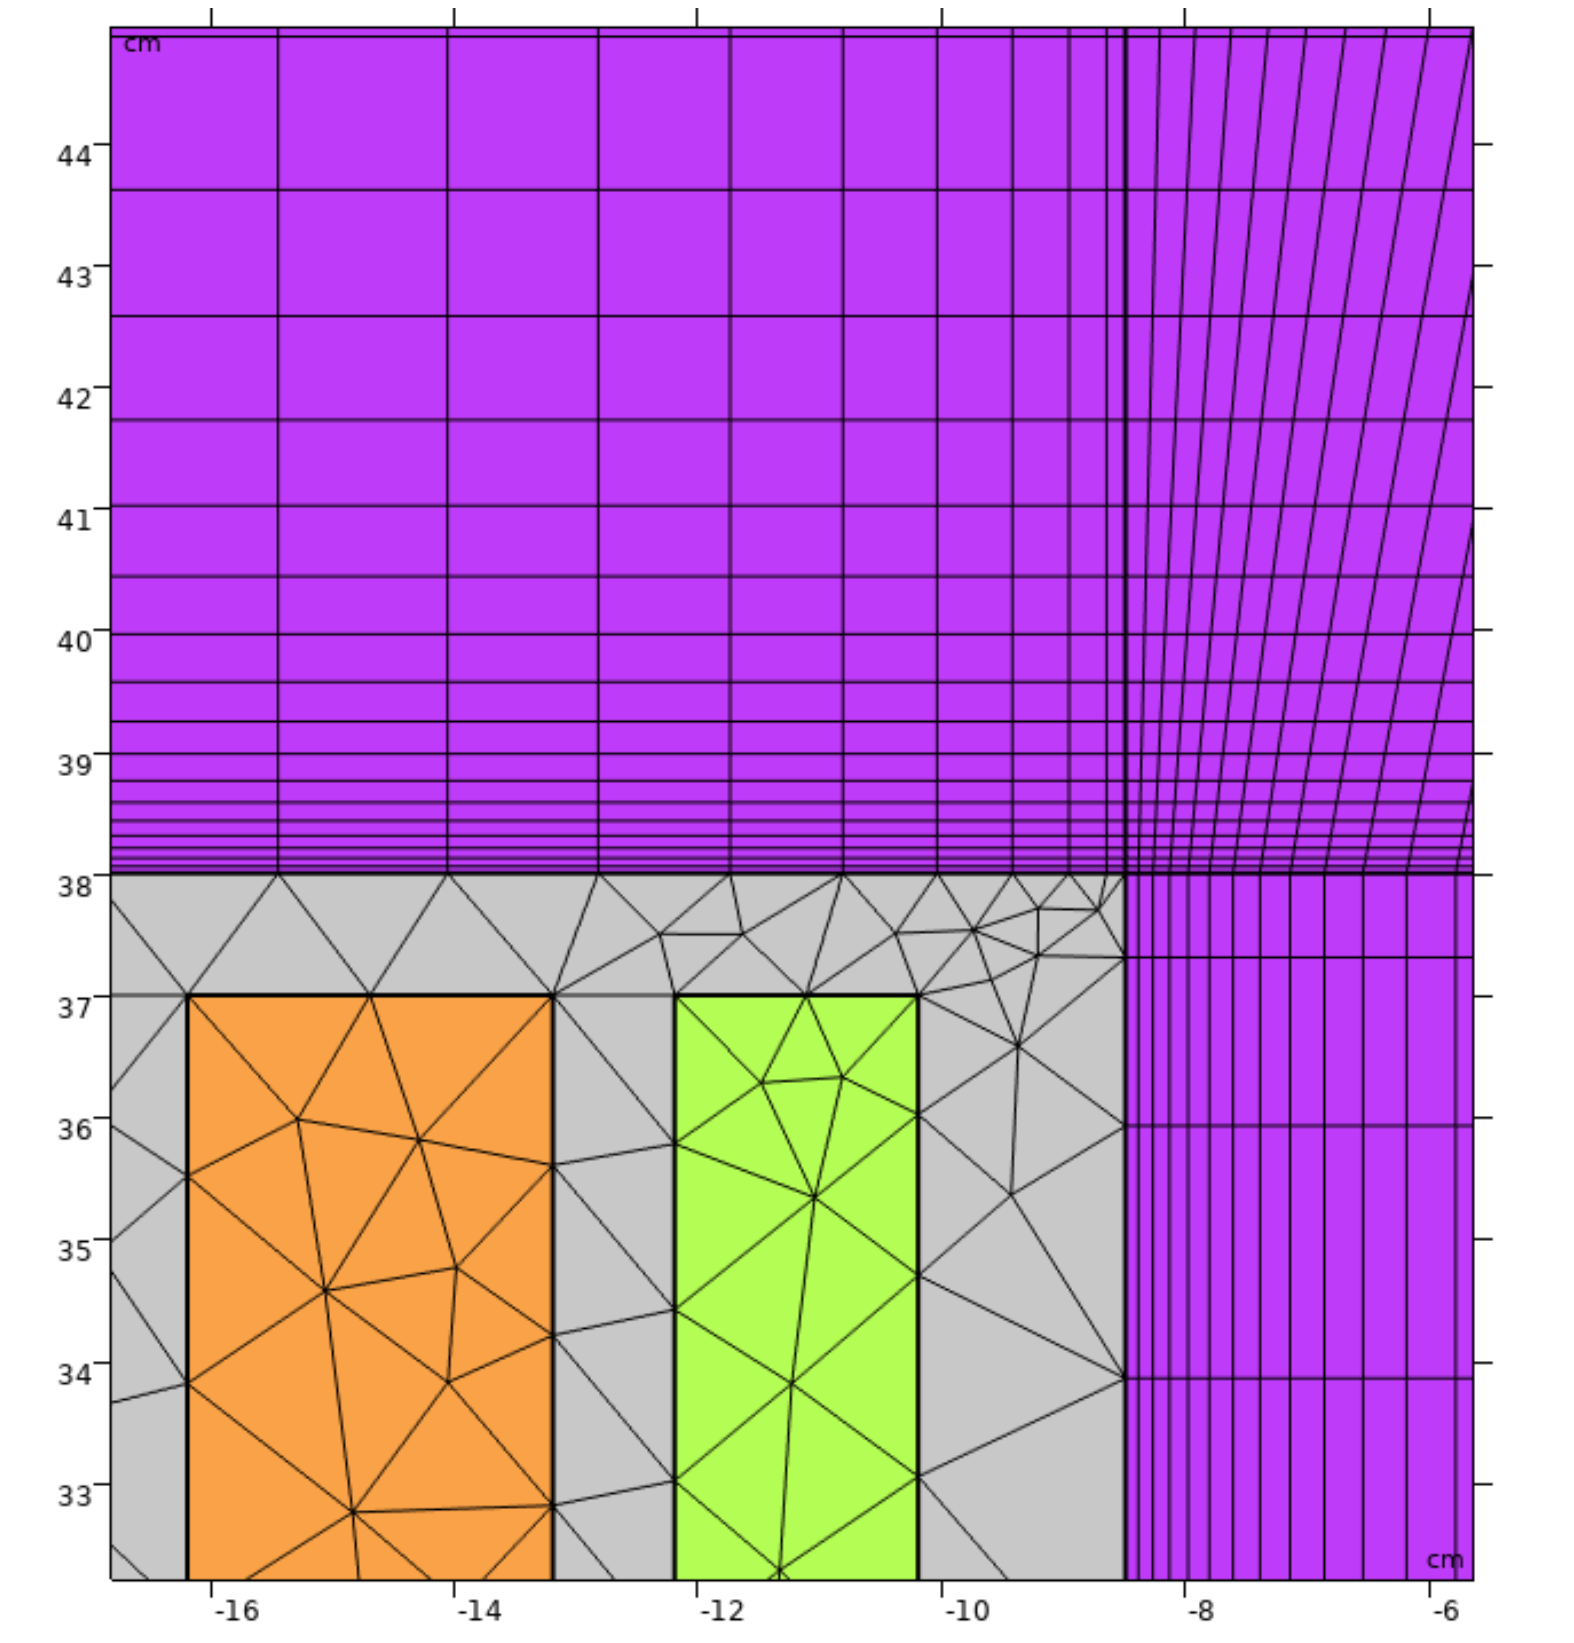
\includegraphics[width=0.45\textwidth]{img/hybrid_mesh.png}
    \end{multicols}
    \caption{Hybrid mesh that can be used to accurately model the skin effect (\cite{vanDijk2022}).}
    \label{fig:mesh_hybrid}
\end{figure}



\subsection{Single frequency}
One possible assumption is that, because the current has a constant frequency, $A_z$ also has one frequency. 
Then, separation of variables is valid, and we can write
\begin{align*}
    u(x,y,t) = \hat u(x,y) \cdot e^{j\omega t}.
\end{align*}
This means that $\frac{\partial}{\partial t} \to \omega j$. The new system is then
\begin{equation}
    \sigma j \omega \hat u = \nabla \times \left[\frac{1}{\mu}\nabla \hat u\right] + f,
\end{equation}
met de weak form
\begin{equation*}
    \left[\sigma \omega j M + \frac{1}{\mathbf \mu}A\right]\hat u = \hat f.
\end{equation*}

\subsection{Meerdere frequenties}
De aanname dat er één frequentie is, is niet geldig. STEDIN meet namelijk dat dit niet het geval is. We kunnen het probleem ook opsplitsen in meerdere frequenties:
\begin{equation}
    u(x,y,t) = \hat u_1(x,y) e^{j\omega_1 t} + \hat u_2(x,y) e^{j\omega_2 t} + \dots.
\end{equation}

\subsubsection{Superpositie}
Als we aannemen de frequenties elkaar niet beïnvloeden, kunnen we $\hat u_1(x,y)$ en $\hat u_2(x,y)$ apart oplossen.

\subsubsection{Gekoppeld}
De aanname dat de frequenties elkaar niet kunnen beïnvloeden is echter niet juist. De permeabiliteit $\mu$ hangt namelijk af van $\text{grad} \; u$. In werkelijkheid is dit systeem dus gekoppeld. Hoe reken je tegelijkertijd meerdere frequenties door? Dit roept de vraag op of het dan toch niet beter is om het probleem direct op te lossen.

\section{Naar het systeem}

We hebben de volgende weak form afgeleidt:
\begin{equation}
    \sigma M \dot u = \frac{1}{\mu}A u + f.
\end{equation}
Dit willen we transformeren in een systeem van vergelijkingen. De stiffness matrix $A$.

\begin{align*}
    \int_{\Omega_e} \nabla \times \left(\frac{1}{\mu} \nabla \times \hat u\right) d \Omega \\
    \omega = \sum_i c_i B_i\\
    \hat u = \sum_j c_j \hat B_j
\end{align*}

Kunnen we het ook zonder numerieke integratie doen (dus analytisch)? En anders, welke ... integratie rule gebruiken we? (Gauss-Legendre)

Antwoord Philip: Je hebt een library sympy om dat te doen. Dat rekent de basis functions analytisch uit.

\section{De matrix M}

Voor het element $e_k$:
\begin{align*}
    M_{e_k} = \left[\int_{\Omega_{e_k}}\phi_i\phi_jdxdy\right]_{1 \leq i, j \leq 3}
\end{align*}

We gaan deze matrix diagnoaal maken. Door een approximatie (kwadratuur?)
\begin{align*}
    \int_{\Omega_e}g(x,y)dxdy \approx (\text{area}) \cdot (\text{gemiddelde waarde}) \\
    \left[\phi_i\phi_j\right]_{i \leq i,j \leq 3} = I_{3 \times 3}
\end{align*}

Voor de $f$ doen we hetzelfde.


\end{document}